\chapter{シミュレーション}

\section{電磁界シュミレータ}
今回電磁界解析シュミレーターを用いて空洞共振器の設計を行った。使用したシュミレーターはMW-Studio(CST社)\cite{CST}であり、このシュミレーターの解析モードは以下の2つである。\cite{MWS-1}

\subsection{固有値解析}
固有値解析モードでは、共振器の構造や材質から、共振器内の電磁場分布をMaxwell方程式の固有値解析から求めるモードである。様々な共振周波数に対応する電磁場の空間分布を把握する事ができる。今回は、共振器の構造とから、共振モードとその電磁場分布、共振周波数を知るために使用する。

\subsection{過渡解析(トランジェント解析)}
過渡解析(トランジェント解析とも)モードでは、共振器内にマイクロ波パルスを入力し、その応答をフーリエ変換して周波数特性を解析するモードである。透過特性の解析には、マイクロ波を入射するためのポートと透過波を取り出すポートを設定する必要がある。トランジェント解析モードは、共振器と外部との伝送路の結合条件を解析するために用いる。

\subsection{有限積分法}
また今回のシュミレーターMW-StudioはFIT(有限積分法)を用いている。\cite{MWS-2}FITは普遍的な空間分散スキームを擁する数値解析手法であり、
T.Weilandにより初めて提唱された\cite{FIT}ものである。
FITは他の多くの数値解析手法のような微分形式ではなく、
以下のような積分形式のマクスウェル方程式を離散化して計算を行う。

\begin{eqnarray}
  \oint_{\partial A} \mathbf{E} \cdot d\mathbf{s}
  = - \int_{\partial A} \frac{\partial \mathbf{B}}{\partial t} \cdot d  \mathbf{A}\\
  \oint_{\partial A} \mathbf{H} \cdot d\mathbf{s} =  \int_{\partial A} \{ \frac{\partial \mathbf{D}}{\partial t} + \mathbf{J} \} \\
  \oint_{\partial V} \mathbf{D} \cdot d\mathbf{A} = \int_V \rho dV \\
  \oint_{\partial V} \mathbf{B} \cdot d\mathbf{A} = 0
\end{eqnarray}

これらの方程式を解く際には、最初に解析対象を包含する有限の計算領域を定義する必要がある。次にこの良識を適切なメッシュシステムによって多くの小さなグリットセルに分割する。

\vspace{10 mm}

\begin{figure}[h]
  \begin{center}
    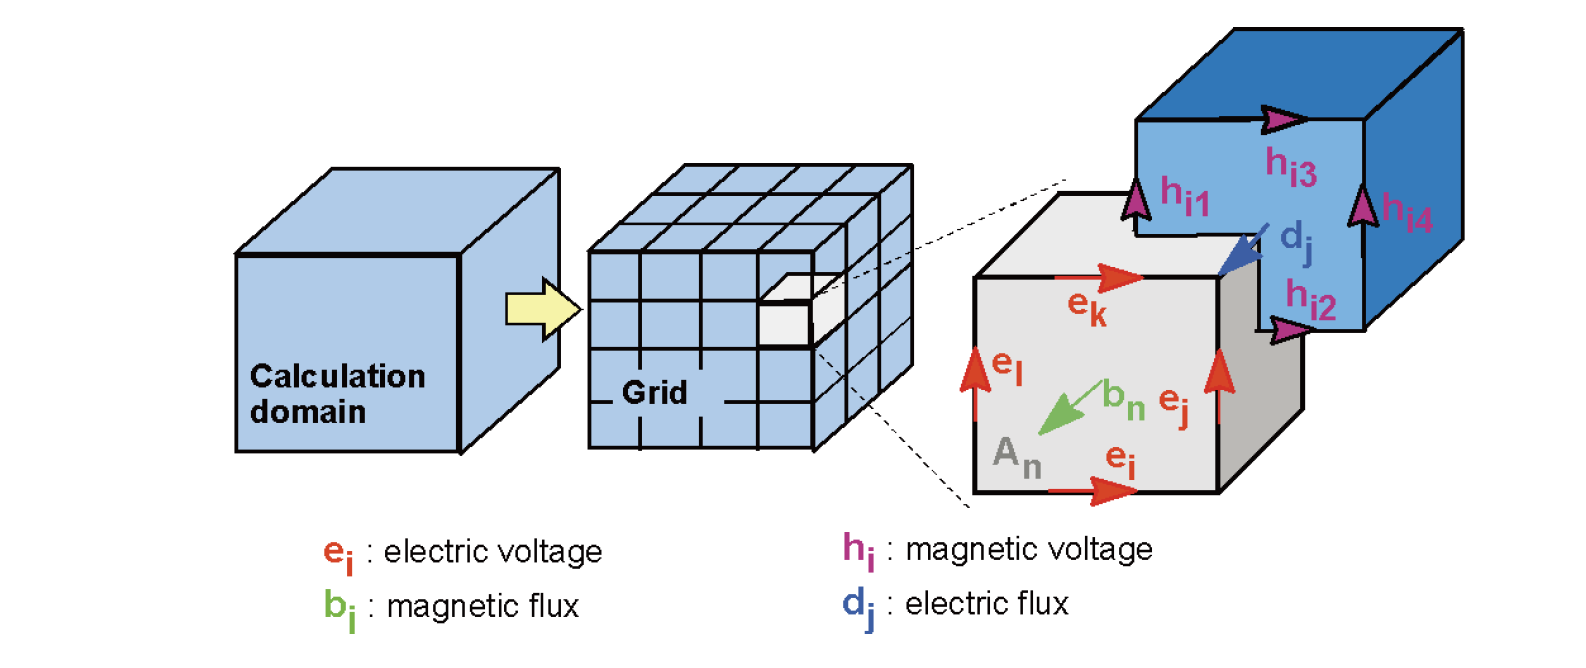
\includegraphics[width=12cm]{./image/mesh.png}
    \caption{メッシュへの分割}
    \label{fig:Mesh}
  \end{center}
\end{figure}

このグリットセルごとに個別のマクスウェル方程式がたつ。つまり、このメッシュの数が計算精度に大きく関わり、メッシュ数をあげればあげるほど精度は高くなるが、計算時間も長くなっていく。

過去の結果から、メッシュ数を細かくしても微細加工をした超伝導素子を置いた時の応答を調べることはできず、実際に製作した場合にシュミレーターと全く同じ条件で行うことはできないため、誤差があることは承知した上で、シュミレーションを行った。また、メッシュ数が2000程度の場合、共振周波数の計算値とのズレは1GHz以下であった。

\section{シュミレーションの設定}
シュミレートの基本設定以下に記す

\begin{itemize}
  \item メッシュ数20000前後
  \item 空洞を構成する素材は完全導体
  \item 周波数範囲30 〜 80GHz
  \item Accuracyは-40dB
\end{itemize}

Accuracyというのは、解析空間内の電磁界エネルギーの総量が設定した値まで減衰したら計算を終了する設定である。解析周波数範囲によりシミュレーションする周波数の刻みが変わり、解析周波数範囲が大きいほど刻みも大きくなり、解析周波数範囲が小さいと刻みも小さくなる。
